\section{Zielsetzung}
\label{sec:Zielsetzung}
Ziel dieses Versuchs ist es die diskreten Energiewerte der Elektronenhülle des Hg-Atoms zu untersuchen.
Dafür wird die integrale Energieverteilung der beschleunigten Elektronen bei zwei unterschiedlichen Temperaturen untersucht. 
Außerdem werden zwei Franck-Hertz-Kurven für zwei weitere Temperaturen aufgenommen.

\section{Theorie}
\label{sec:Theorie}
Für die Strukturaufklärung der Elektronenhülle müssen Elektronstoßexperimente durchgeführt werden.
Dazu werden Elektronen mit geeigneter Energie auf Atome geschossen. Die entstehenden Energieverluste der Elektronen liefern Informationen über die
Struktur.

\subsection{Aufbau und Ablauf des Franck-Hertz Experimentes}
\label{subsec:AufAbTheo}
Die Apparatur vom Franck-Hertz-Versuch ist schematisch in \autoref{fig:Abb_1} dargestellt.
\begin{figure}[H]
    \centering
    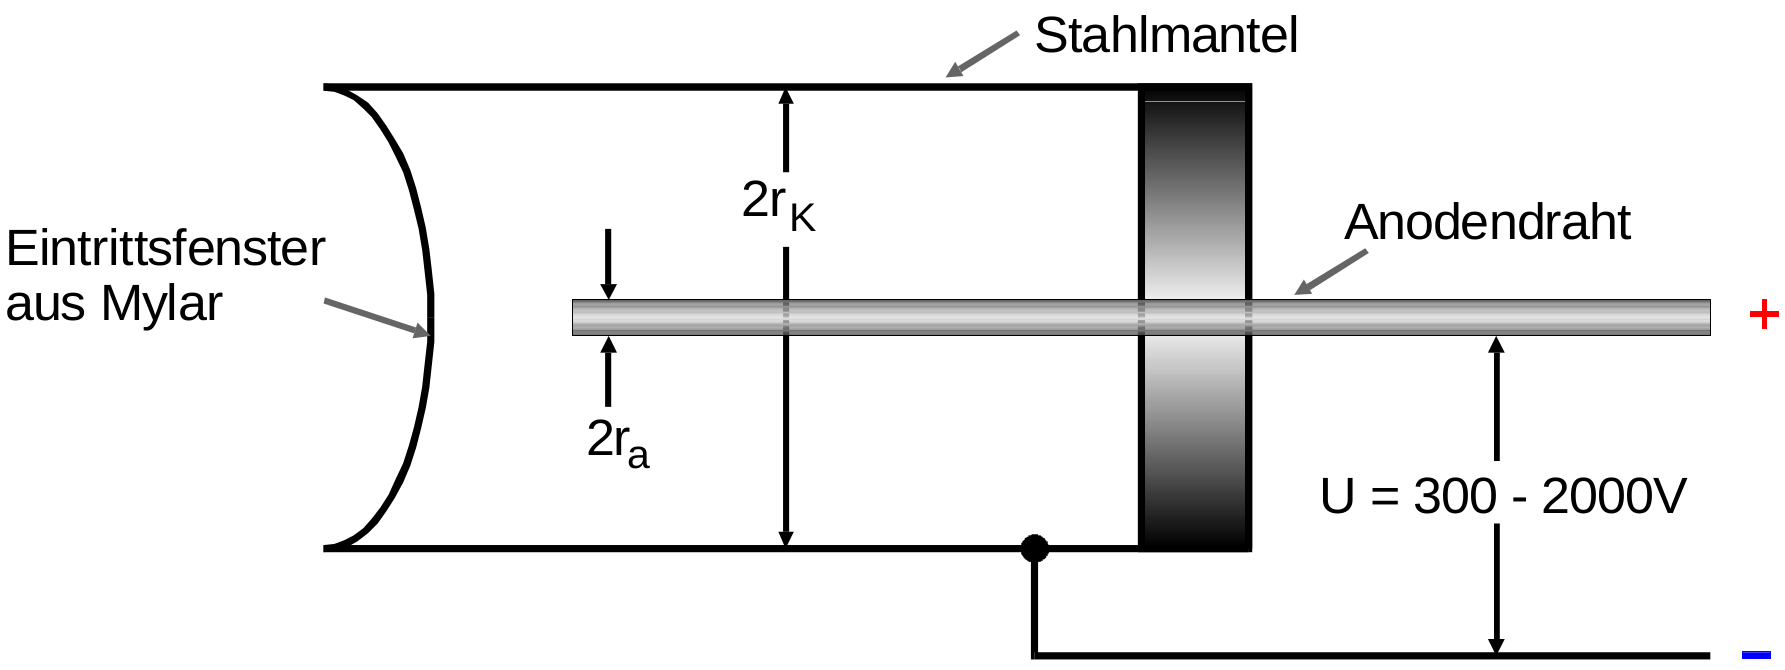
\includegraphics[width=0.6\textwidth]{build/Abb_1.png}
    \caption{Schematische Darstellung des Franck-Hertz-Versuchs\cite{V601}.}
    \label{fig:Abb_1}
\end{figure}
Der Aufbau besteht aus einer evakuierten Röhre, in der ein Quecksilber-Tropfen ist, welcher spontan verdampft. Dadurch stellt sich ein 
Gleichgewichtsdruck $p_{s\ddot{a}t}$ ein, wobei die Dampfdichte von der Umgebungstemperatur $T$ abhängt.
Auf der einen Seite der Röhre befindet sich ein negativ geladener Glühdraht, der mit einem Material beschichtet ist, welches eine besonders geringe
Austrittsarbeit besitzt. Durch den glühelektrischen Effekt werden möglichst viele freie Elektronen erzeugt.
Diese Elektronen werden zu einer positiv geladenen Gitterelektrode hin beschleunigt. Dabei liegt zwischen Gitter und Draht eine Beschleunigungsspannung
$U_B$ an. Aufgrund der Energieerhaltung gilt nach dem Durchlaufen des Feldes
\begin{equation*}
    \frac{m_0}{2} v^2_{vor} = e_0 U_B,
\end{equation*}
wenn die Elektronen zu Beginn eine Geschwindigkeit von Null besitzen.
Hinter der Gitterelektrode befindet sich eine negativ geladene Auffängerelektrode und dazwischen liegt eine Bremsspannung $U_A$ an.
Dies führt zu einem Gegenfeld, welches die Elektronen überwinden müssen, um die Auffängerelektrode erreichen. An dieser wird ein Auffängerstrom
$I_A$ gemessen. Es kommen nur Elektronen an, deren Energie groß genug ist um das Gegenfeld zu passieren.\\
Im Bereich zwischen Glühdraht und Gitterelektrode kann es zu Stößen zwischen Elektronen und Hg-Atomen kommen. Abhängig von der Beschleunigungsspannung
$U_B$ wird zwischen zwei Möglichkeiten unterschieden.\\
Die eine Methode ist, dass nur elastische Stöße auftreten, was passiert, wenn die Energie der Elektronen bei niedriger Beschleunigungsspannung noch nicht groß genug ist.
Beim elastischen Stoß wird nicht viel Energie abgegeben, es kommt zu einer Richtungsänderung. Die Energie, die beim elastischen Stoß übertragen wird beträgt
\begin{equation*}
    \Delta E = \frac{4m_0M}{(m_0 + M)^2} E \approx 1,1 \cdot 10^{-5} E,
\end{equation*}
wobei $m_0$ die Elektronenmasse und $M$ die Hg-Atommasse ist.\\
Die zweite Möglichkeit geschieht, wenn die Energie der Elektronen durch eine größere Beschleunigungsspannung groß genug ist, 
sodass sie die Hg-Atome anregen können. Es wird der Energiebetrag $E_1-E_0$ vom beschleunigten Elektron auf ein Elektron in einer inneren Hülle des Hg-Atom übertragen.
Dabei behält das Elektron eine Restenergie und das Hg-Atom kehrt nach einer Relaxationszeit von ca. $10^{-8}\si{\second}$ in den Grundzustand zurück 
und ein Photon mit der Energie
\begin{equation}
    E_{Photon} = h \nu = \frac{hc}{\lambda} = E_1 - E_0
    \label{eqn:Anregungspotential}
\end{equation}
wird emittiert.
Immer wenn die Energie des Elektrons größer oder gleich der Anregungsenergie ist, hat
es nach dem inelastischen Stoß nicht mehr genug Restenergie, um das Gegenfeld zwischen
Gitter- und Auffängerelektrode zu überwinden, wodurch der Auffängerstrom sinkt.
Die Abhängigkeit des Auffängerstroms zur Beschleunigungsspannung unter idealen Bedingungen wird in \autoref{fig:Abb_2} dargestellt.
\begin{figure}[H]
    \centering
    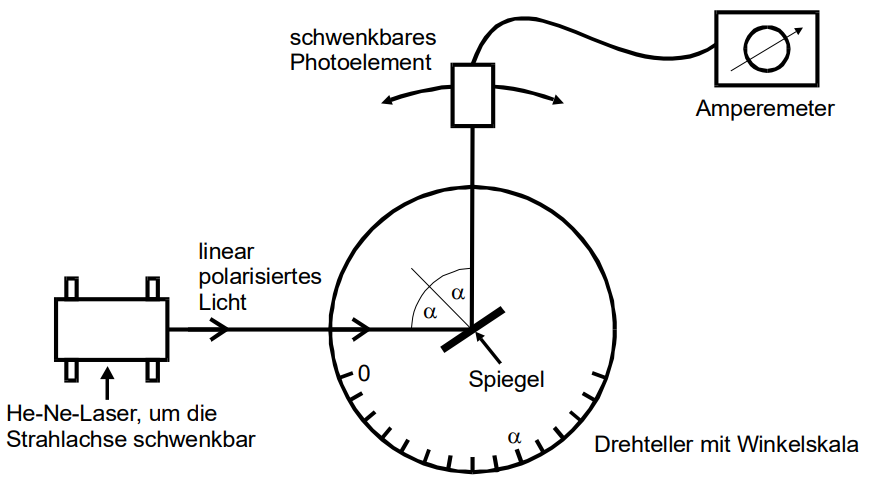
\includegraphics[width=0.4\textwidth]{build/Abb_2.png}
    \caption{Idealisierter Verlauf der Franck-Hertz-Kurve\cite{V601}.}
    \label{fig:Abb_2}
\end{figure}
Zu Beginn ist die Beschleunigungsspannung noch gering, sodass keine Elektronen das Gegenfeld überwinden können, weswegen der Auffängerstrom gleich 
Null ist. Bei steigender Beschleunigungsspannung besitzen mehr Elektronen die benötigte Energie um die Auffängerelektrode zu erreichen, wobei der Strom $I_A$
steigt. Der Strom nimmt mit steigender Beschleunigungsspannung bis zu dem Punkt zu, an dem diese einen Wert von $U_1$ erreicht hat und die 
Elektronen die Energie $E_1 - E_0$ besitzen. Der Auffängerstrom nimmt ab, da die Hg-Atome angeregt werden. 
Wenn die Beschleunigungsspannung nun weiter steigt, haben die Elektronen schneller
die zum Anregen der Hg-Atome nötige Energie und die (im gegebenen Versuchsaufbau nicht
sichtbare) Leuchtschicht wandert in Richtung des Glühdrahts. Zudem haben auch mehr
Elektronen genug Energie, um das Gegenfeld zu überwinden, sodass auch die Peaks in
der Stromstärke zunehmend intensiver werden.
Dieser Vorgang wird periodisch fortgesetzt, wobei der Spannungsabstand $U_1$ einen Zusammenhang  mit der Anregungsenergie der Hg-Atome beitzt nämlich
\begin{equation*}
    U_1 = \frac{1}{e_0} (E_1 - E_0)\label{eqn:Grundzustand}
\end{equation*}
mit der Elektronenladung $e_0$.

\subsection{Einflüsse auf die Gestalt der Franck-Hertz-Kurve}
\label{subsec:Franck-Hertz-Kurve}
Der idealisierte Verlauf der Franck-Hertz-Kurve kann nicht realisiert werden, weil verschiedene Nebeneffekte beachtet werden müssen.
Diese beeinflussen den Verlauf der Kurve.

\subsubsection{Das Kontaktpotential}
\label{subsubsec: Kontaktpotential}
Ein Nebeneffekt kommt dadurch zustande, dass sich das Potential des Glühdrahtes von dem der Gitterelektrode unterscheidet.
Die Messung würde verfälscht werden, wenn bei gleichem Potential und bei steigender Temperatur auch aus der Gitterelektrode Elektronen austreten.
Deshalb wird der Glühdraht so beschichtet, dass er eine geringere Austrittsarbeit als die Gitterelektrode aufweist.
\begin{figure}[H]
    \centering
    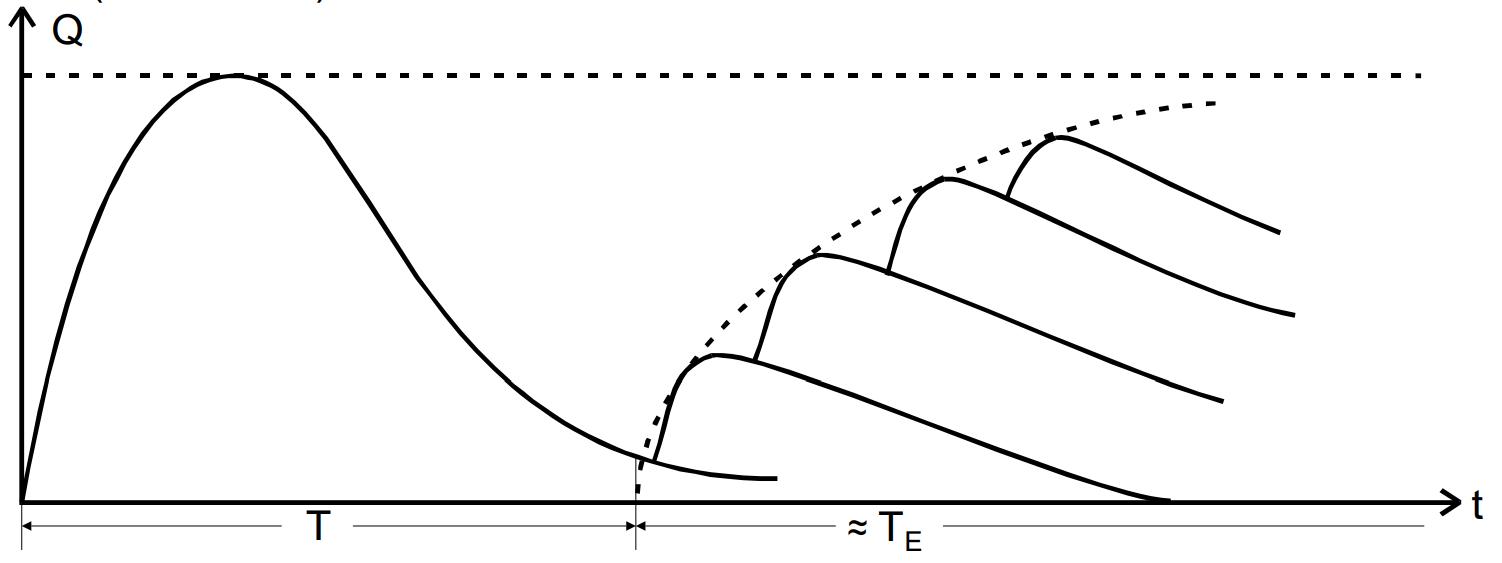
\includegraphics[width=\textwidth]{build/Abb_3.png}
    \caption{Das Verhältnis zwischen dem Potential des Glühdrahtes und der Gitter-
    elektrode\cite{V601}.}
    \label{fig:Abb_3}
\end{figure}
Das Potentialverhältnis wird in \autoref{fig:Abb_3} dargestellt, wobei die Größen $\phi_G$ und $\phi_B$ die Austrittsarbeiten des Glühdrahts und
der Gitterelektrode sind.
Das Kontaktpotential 
\begin{equation*}
    K = \frac{\phi_B}{e_0} - \frac{\phi_G}{e_0}
    \label{eqn:Kontaktpotential}
\end{equation*}
ergibt sich aus dem Potentialverhältnis, womit sich eine Verschiebung nach
\begin{equation}
    U_{B,eff} = U_B - K
    \label{eqn:Verschiebung}
\end{equation}
ergibt.

\subsubsection{Die Energieverteilung der Elektronen}
\label{subsubsec:Energieverteilung}
Der nächste Nebeneffekt entsteht durch die Fermi-Dirac-Verteilung der Elektronen im Glühdraht. Diese besagt, dass sich das Elektron schon vor dem
Herauslösen auf verschiedenen Energieniveaus befinden, weswegen sie unterschiedliche Anfangsgeschwindigkeiten haben, wenn sie aus dem Draht gelöst werden.
Deswegen haben sie nach der Beschleunigung ein kontinuierliches Energiespektrum.\\
Der Abstand zwischen den Strommaxima ist nicht einheitlich, weil die Beschleunigung der Elektronen nicht gleich stark ist. Aus diesem Grund wird auch der Auffängerstrom nicht mehr
ganz auf Null abfallen, sondern immer nur einen Minimalwert erreichen.\\
\\
Die Richtungsänderung der Elektronen bei den elastischen Stößen im Bereich zwischen der Gitterelektrode und der Auffängerelektrode ist relevant,
weil somit die Elektronen die Auffängerelektrode nicht mehr erreichen können.

\subsubsection{Der Dampfdruck}
\label{subsubsec:Dampfdruck}
Der Dampfdruck $p_{s\ddot{a}t}$
\begin{equation}
    p_{s\ddot{a}t}(T) = 5,5 \cdot 10^7 exp(\frac{-6876}{T})
    \label{eqn:psät}
\end{equation}
hat auch einen Einfluss auf die Franck-Hertz-Kurve. Zur Messung der Franck-Hertz-Kurve sind inelastische Stöße benötigt,
welche nur Zustande kommen, wenn die mittlere Weglänge
\begin{equation}
    \bar{\omega} = \frac{0,0029}{p_{s\ddot{a}t}}
    \label{eqn:Weglänge}
\end{equation}
klein gegenüber dem Abstand $a$ zwischen Glühdraht und Gitterelektrode ist. Hier gilt $a = 1 \si{\centi\meter}$.
Der Dampfdruck ist hauptsächlich abhängig von der Temperatur $T$, was in \autoref{fig:Abb_4} dargestellt ist.
\begin{figure}[H]
    \centering
    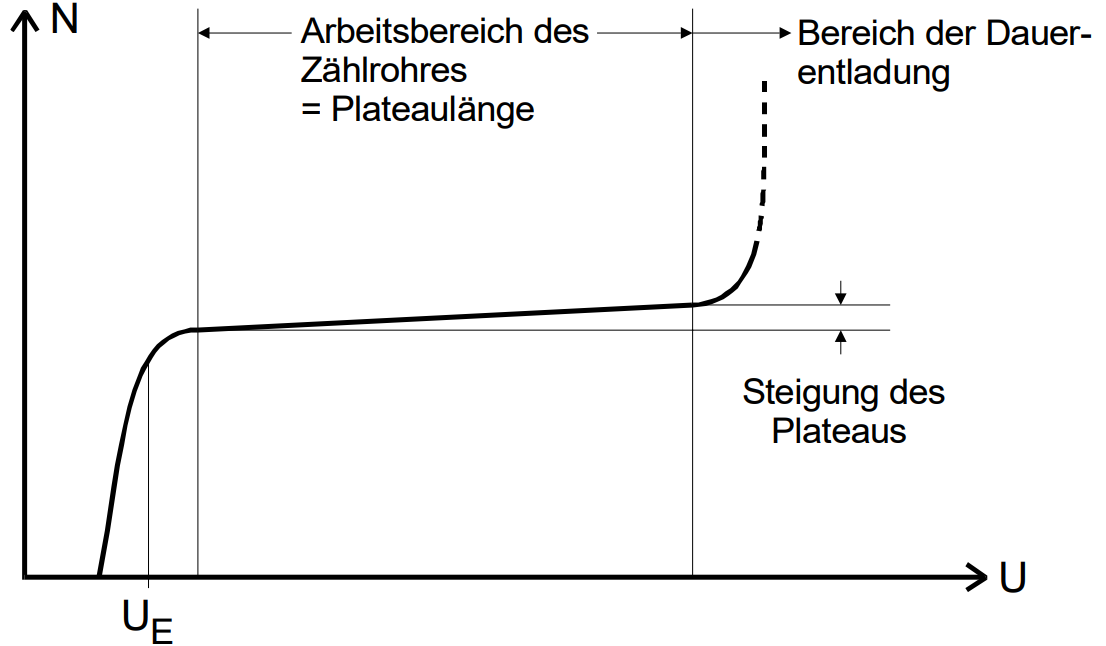
\includegraphics[width=0.6\textwidth]{build/Abb_4.png}
    \caption{Abhängigkeit des Dampfdrucks von Hg von der Temperatur\cite{V601}.}
    \label{fig:Abb_4}
\end{figure}
